\chapter*{Anexos}
\addcontentsline{toc}{chapter}{Anexos}

\section{Matriz de evaluacion de madurez BIM}

\begin{figure}[H]
    \centering
    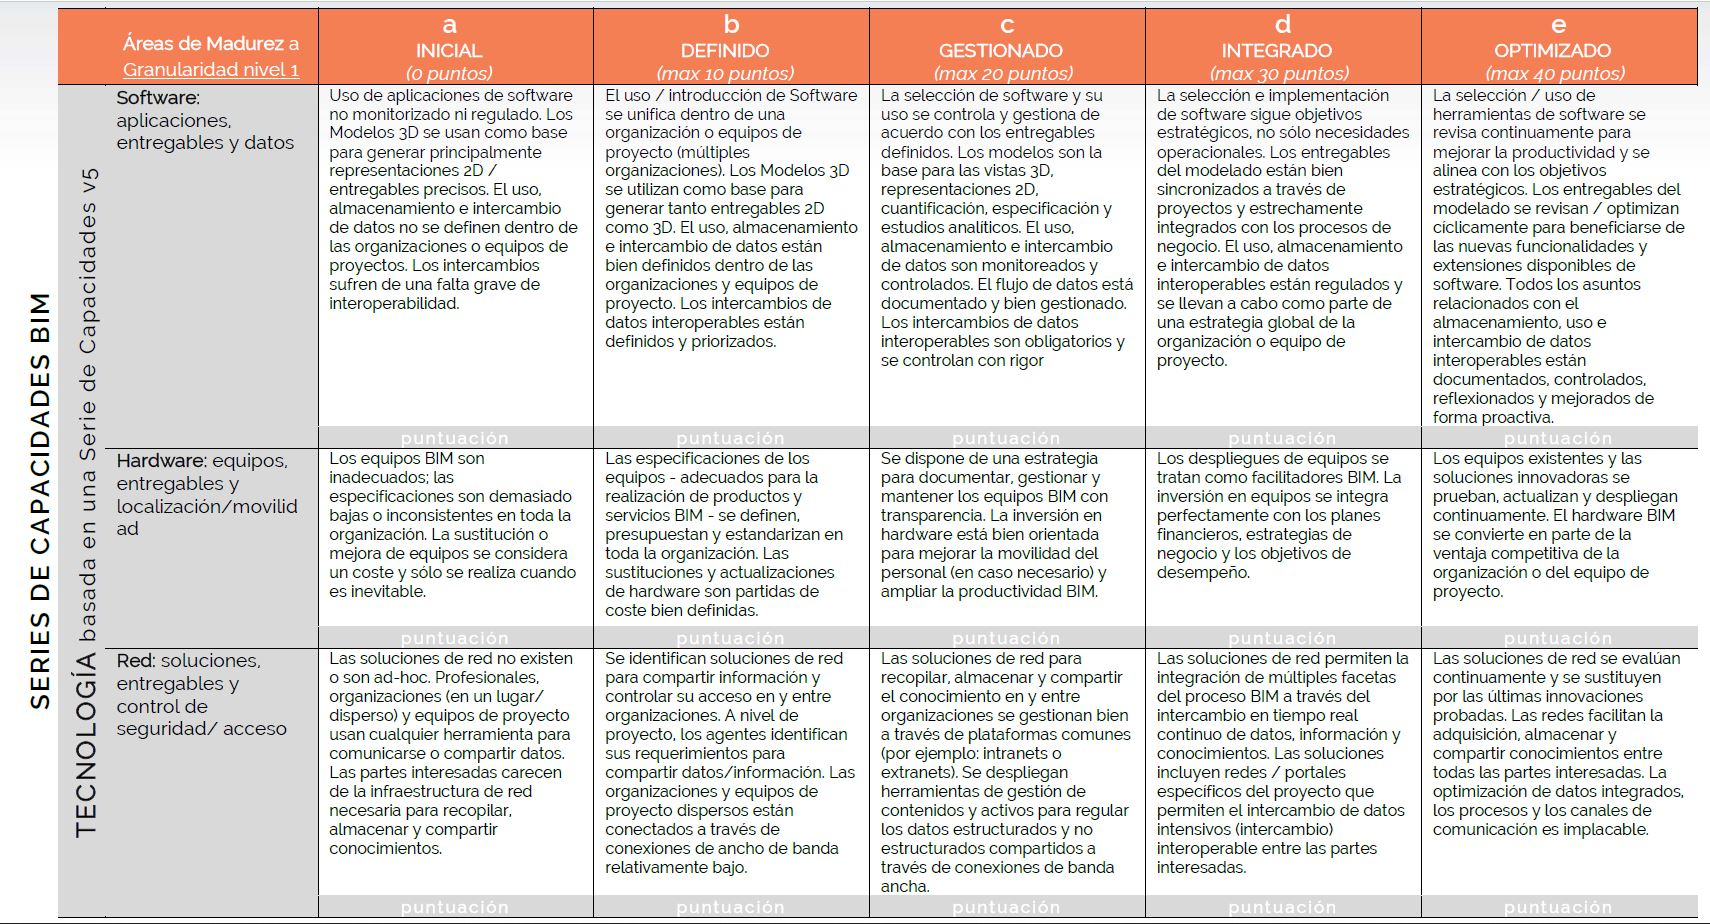
\includegraphics[width=1\linewidth]{images/matriz-madurez-1.jpeg}
    \caption{Matriz basada en la teconología.}
\end{figure}

\begin{figure}[H]
    \centering
    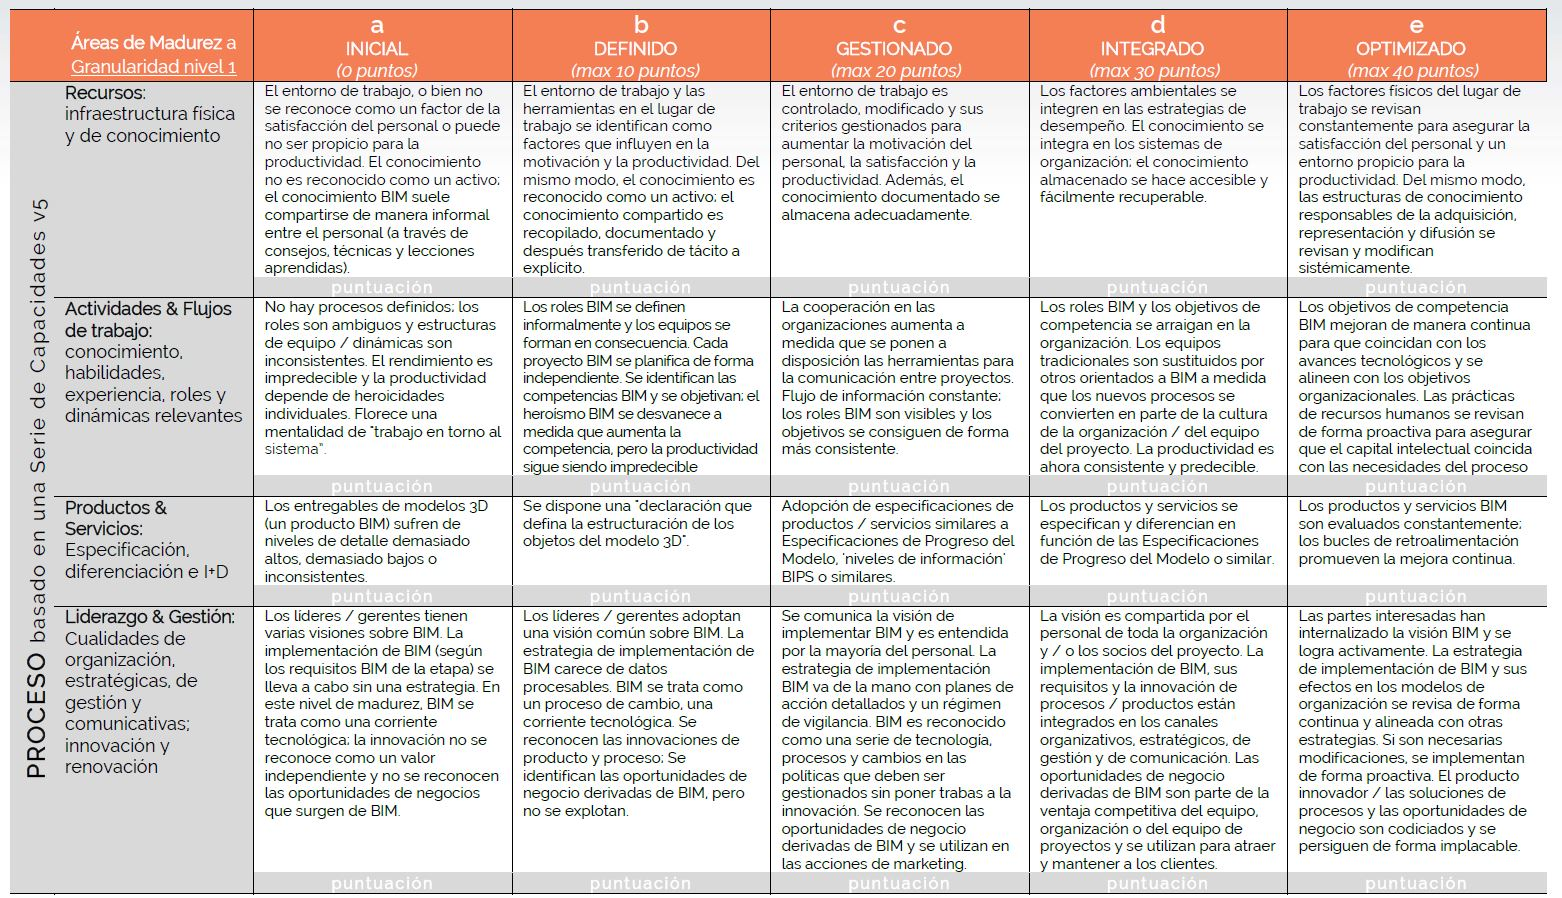
\includegraphics[width=1\linewidth]{images/matriz-madurez-2.jpeg}
    \caption{Matriz basada en el proceso.}
\end{figure}

\begin{figure}[H]
    \centering
    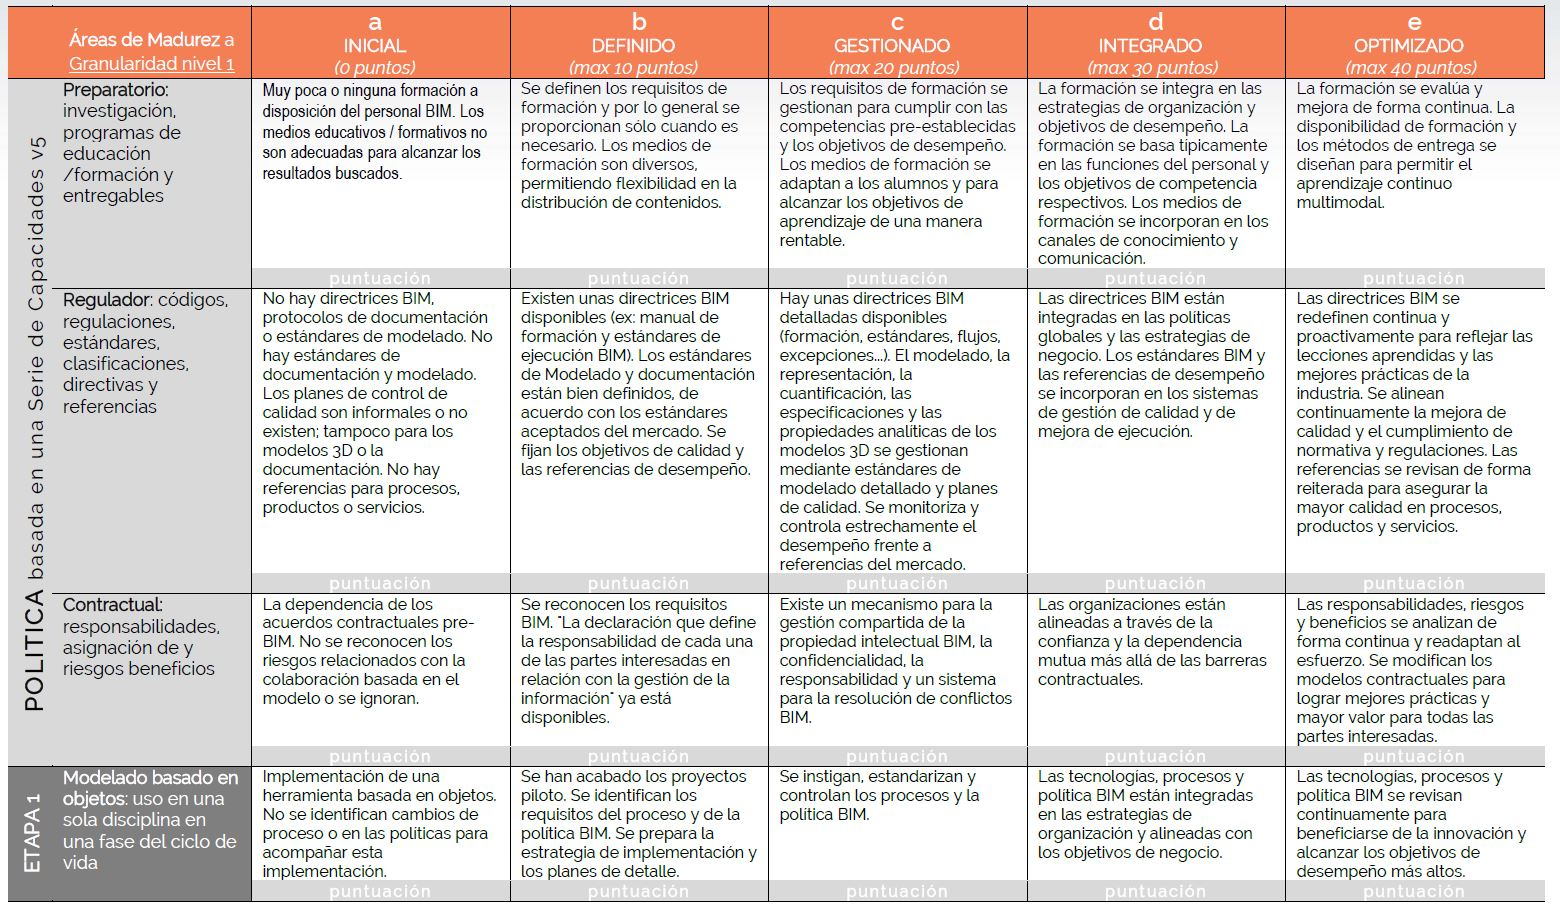
\includegraphics[width=1\linewidth]{images/matriz-madurez-3.jpeg}
    \caption{Matriz basada en la política.}
\end{figure}

\section{Códigos de los desarrollos}

\subsection{Herramienta de transformación de la data}

\begin{lstlisting}[language=Python]
import pandas as pd
import numpy as np
import os, glob

data = input('Nombre archivo:')
monto = float(input('Monta base:'))
variacion = float(input('Variacion:'))

def contracts(data, monto, variacion):
    path = (os.getcwd() + '/data/' + data).replace('\\','/')
    df = pd.read_excel(path, header=7)
    df.drop(df.columns[[1,2,4,5,6,7,8]], axis=1, inplace=True)
    df.columns = ['Contrato', 'Descripcion', 'Total']
    df.dropna(subset=['Total'], how='any', inplace=True)

    contrato = (df[df['Contrato'].str.contains('nombre', case=False)]
                                 .iloc[:,0])
                                 .reset_index(drop=True)
    base = (df[df['Contrato'].str.contains('revision 0.0', case=False)]
                             .iloc[:,2])
                             .reset_index(drop=True)
    cierre = (df[df['Contrato'].str.contains('total compro', case=False)]
                               .iloc[:,2])
                               .reset_index(drop=True)

    df1 = pd.concat([contrato, base, cierre], axis=1)
    df1.columns = ['Contrato', 'Base', 'Cierre']
    df1['Delta'] = df1['Cierre'] - df1['Base']

    #Remueve los primeros 8 caracteres del string en la columna 'Contratos'
    df1['Contrato'] = df1.Contrato.str.slice(start=8) 
    df1['Variacion'] = df1['Delta']/(df1['Base'] + 0.00000001)

    df2 = df1[df1.Delta > 0].reset_index(drop=True)
    
    df3 = (df2[(df2['Base'] > monto) & (df2['Variacion'] > variacion)])
                .sort_values(by=['Base'], ascending=False)
                .reset_index(drop=True)

    return df, df1, df2, df3

df, df1, df2, df3 = contracts(data, monto, variacion)

def contract_analysis_base(df, monto, variacion):

    dfs = df[df.Contrato.str.match('0.0|nombre|revision 0.0|total compro', 
                                   case=False)]
                                   .reset_index(drop=True)
    dfs[dfs['Descripcion'].str.contains('suministr', 
                                         case=False)==True]

    ind_nombre = dfs[dfs['Contrato'].str.contains('nombre', 
                                                   case=False)]
                                    .index
                                    .tolist()
    ind_base = dfs[dfs['Contrato'].str.contains('revision 0.0', 
                                                 case=False)]
                                  .index
                                  .tolist()
    ind_cierre = dfs[dfs['Contrato'].str.contains('total compro', 
                                                  case=False)]
                                    .index
                                    .tolist()
    ind_df = pd.DataFrame(np.column_stack([ind_nombre, 
                                        ind_base, 
                                        ind_cierre]), 
                                        columns=['indice contrato', 
                                                 'indice base', 
                                                 'indice cierre'])

    l = []
    for i in range(len(ind_df)):
        if (dfs.Total[ind_df['indice base'][i]] > monto) 
            and 
           (dfs.Total[ind_df['indice cierre'][i]] /
           dfs.Total[ind_df['indice base'][i]] - 1 > variacion):

            s = dfs.iloc[ind_df['indice contrato'][i]
                    :ind_df['indice base'][i], :]
            l.append(s)
            dfx = pd.concat(l, ignore_index=True) 
        
    return dfx

df_base = contract_analysis_base(df, monto, variacion)

def contract_selection(df, monto, variacion):

    df4 = (df[~df['Contrato']
            .str.match('0.0|totales fina', case=False)])
            .reset_index(drop=True) 

    ind_nombre = df4[df4['Contrato']
                .str.contains('nombre', case=False)]
                .index.tolist()
    ind_base = df4[df4['Contrato']
                .str.contains('revision 0.0', case=False)]
                .index.tolist()
    ind_cierre = df4[df4['Contrato']
                .str.contains('total comprom', case=False)]
                .index.tolist()
    ind_df = pd.DataFrame(np.column_stack([ind_nombre, 
                                          ind_base, 
                                          ind_cierre]), 
                            columns=['indice contrato', 
                                     'indice base', 
                                     'indice cierre'])

    l = []
    for i in range(len(ind_df)):
        if (df4.Total[ind_df['indice base'][i]] > monto)
            and (df4.Total[ind_df['indice cierre'][i]]/
                df4.Total[ind_df['indice base'][i]] - 1 > variacion):
            s = df4.iloc[ind_df['indice contrato'][i]
                    :ind_df['indice cierre'][i]+1, :]
            l.append(s)
            df5 = pd.concat(l, ignore_index=True) 

    df5['Contrato'] = df5.Contrato
                         .str.replace('Revision 0.0 - Totales', 
                                      'Costo Base',
                                       regex=False)
    df5['Contrato'] = df5.Contrato
                         .str.replace('Total Compromiso', 
                                      'Costo Final', 
                                       regex=False)
    df5 = df5[~df5.Contrato
                  .str.contains('revision', case=False)]
    return df5

df_s = contract_selection(df, monto, variacion)

resumen = df_s[df_s.Contrato
                   .str.contains('nombre|costo base|costo final', 
                                case=False)]
del resumen['Descripcion']

with pd.ExcelWriter('selected_contracts_(from code).xlsx') as writer:
    df1.to_excel(writer, 
                sheet_name='Reagrupacion', 
                index=False)
    df2.to_excel(writer, 
                 sheet_name='Solo crecimientos', 
                index=False)
    df3.to_excel(writer, 
                 sheet_name='Seleccionados', 
                 index=False)
    df_s.to_excel(writer, 
                  sheet_name='Detalle seleccionados', 
                  index=False)
    resumen.to_excel(writer, 
                     sheet_name='Resumen seleccionados', 
                     index=False)

items = ['extension plazo', 
         'obras adicionales', 
         'materiales', 
         'ingenieria']

key_words = ['extension plazo|plazo', 
            'montaje|obras adicio|adicional
            |extraordinaria|obraexcav|civil|rellen
            |reempla|reparaci|instalaci', 
            'hormig|piping|caner|tuber|valvula
            |valv|pern|sumin|adqui|estruc|acero', 
            'ingenieri|cambios alcan|ingenieria de terreno
            |ingenieria de terreno'] 

def cost_deviations(df, key_words):
    l = []
    for i in range(len(key_words)):
        a = df[df['Descripcion'].str
                                .contains(key_words[i], 
                                          case=False)==True] 
        l.append(a)
        df = df.merge(l[i].drop_duplicates(), 
                            on=['Contrato', 
                                 'Descripcion', 
                                 'Total'], 
                                 how='left', 
                                 indicator=True)
        df = df[df['_merge'] =='left_only']
        del df['_merge']

    return l

l = cost_deviations(df_s, key_words)

def resumen_items(l, items):
    d = {}
    a = 0 
    for i in range(len(items)):       
            d[items[i]] = l[i].Total.sum()
            a += l[i].Total.sum()
            
    d['Total'] = a
    dff = pd.DataFrame(d, index=['USD', 'Var']).T
    dff.Var = dff.USD/df2.Base.sum()

    return dff

dff = resumen_items(l, items)

dx = resumen_items(cost_deviations(df_base, key_words), items)

with pd.ExcelWriter('cost_deviations_(from code).xlsx') as writer:
    dff.to_excel(writer, 
                 sheet_name='Resumen seleccionados', 
                 index=True)
    dx.to_excel(writer, 
                sheet_name='Resumen seleccionados base', 
                index=True)
    for i in range(len(items)):
        pd.DataFrame(l[i]).to_excel(writer, 
                                    sheet_name=items[i], 
                                    index=False)
\end{lstlisting}

\subsection{Herramienta de estimación de los parámetros}

\begin{lstlisting}[language=Python]
import pandas as pd
import statsmodels.api as sm
import os

def main():
    path:str = os.getcwd() + "/data.csv"

    # Matriz de datos globales
    data_df = pd.read_csv(path)
    data_df["indicador_madurez"] = 4 / data_df["madurez_succar"]
    data_df["const"] = 1

    # Matrices Y y X
    y_data = data_df["desv_costos"]
    x_data = data_df[["const", "indicador_madurez"]]

    regression = sm.OLS(endog=y_data, 
                        exog=x_data,
                        missing="drop")
    result_reg = regression.fit()
    result_summary = result_reg.summary()

    print(result_summary)
    print("\nDATA INGRESADA PARA LA ESTIMACION\n")
    print(data_df)

    
if __name__ == "__main__":
    main()
\end{lstlisting}
